\documentclass{article}
\usepackage{graphicx} % Required for inserting images
\usepackage[a4paper, total={6in, 8in}]{geometry}
\usepackage{float}

\title{Parallelism Basics}
\author{}
\date{}

\begin{document}

\maketitle

    Although parallelism may seem like another fancy, confusing word in the world of computing, the concept it entails is actually incredibly prevalent in everyday life. Rarely does one ever see a fast food kitchen run by only one employee. Usually, a whole team of workers keeps the shop running by doing their own tasks. Rarely does one visit a large grocery store with only one checkout line. Most grocery stores have ten or more to keep up with customers' demands. \\

    Computer hardware is actually naturally parallel. It is built to handle multiple tasks at once. However, at the dawn of the computing age, computer architects designed programming languages and tools in a serial way. In other words, programmers for decades were trained to write code that executes sequentially. Each task in such programs is done one after the other. \\

    Serial programs fail to take advantage of continuous improvements in computer hardware, however. As more cores are packed into tiny chips annually, computers become more capable of juggling multiple tasks at the same time. They become excellent multitaskers. Serial programs do not make use of this superpower, however. Thus, their performance stagnates despite incredible increases in processing power being made annually. \\
    
    Why did the founding leaders of the computing age like serial programs so much then? Serial programs are \textbf{deterministic}! Each time they are run, they do the same operations in the same order. At the end, they always provide the same answer given the same inputs. The timing of tasks' execution in parallel programs is not deterministic, however. Thus, one can already foresee one of several main challenges in working with parallel programs. \\

    Some steps of parallel programs must still be run sequentially (step-by-step), however. This is especially when \textbf{dependencies} exist. Two important kinds of dependencies will appear in one's journey through parallelism. \\
\begin{enumerate}
\item \textbf{Data Dependency}\\
Sometimes, a task cannot execute without data produced by another task. For example, at a construction site, the guy in charge of putting in carpets cannot do his job before the woman in charge of making the cement floor has provided him with a solid foundation to furnish.
\item \textbf{Control Dependency}\\
Control dependencies exist when tasks must be ordered as to prevent side effects such as those caused by I/O operations. 
\end{enumerate}
An algorithm's span is the amount of time taken in performing the longest sequential chain of tasks. \\

    The strongest overall strategy for scalable parallelism is \textbf{data parallelism}, the type of parallelism in which data being operated on is split into chunks and each chunk is processed by a different task. More data means more tasks. Thus, data parallelism can scale with input size. The opposite approach is called \textbf{functional decomposition}. In functional decomposition, a program is decomposed into several functions which are run in parallel. Say that a program can be broken into three functions: $f$, $g$, and $h$. At best, if each of these three functions take the same amount of time to run, functional decomposition will only result in three times less time taken to run the program. However, the program's parallelism will not scale with input size. \\

    Furthermore, parallelism can be either \textbf{regular} or \textbf{irregular}. In \textbf{regular} parallelism, tasks being run in parallel are similar and have predictable dependencies. For example, a matrix multiplication is decomposed into a set of dot products. The large task has been turned into a uniform set of tasks that may be run at the same time. Irregular dependencies are those in which tasks are not similar. Their dependencies are unpredictable. 

    Two hardware mechanisms enable parallel computing to happen: \textbf{thread parallelism} and \textbf{vector parallelism}. \\

    In thread parallelism, the task is split among several workers. Each worker has a separate flow of control. Two types of threads exist. A \textbf{hardware thread} is a hardware entity capable of independently executing a program, a flow of instructions. A \textbf{software} thread is a virtual hardware thread. Tasks are organized into software threads which the operating system schedules into hardware threads. \\

    In vector parallelism, the same control flow is used to work on multiple data elements. Single operations (\textbf{vector instructions}) are replicated over collections of data (held in \textbf{vector registers}). Vector registers hold a small array of elements. For instance, Intel's AVX has registers that hold eight thirty-two bit floating point values. Each element is called a \textbf{lane}. \\

    If the definitions provided for both types of threads are confusing, think of the computer like a bakery. Chef Anne needs to spread egg wash on eight dinner rolls. She can do the job serially: pull a roll one-by-one and put egg wash on it. However, the job can be done more quickly in parallel. In thread parallelism, she can give each of her kitchen assistants one roll. They each spread egg wash on their roll, and they return it to Chef Anne. In vector parallelism, she puts all eight rolls in a tray (a vector) and does one operation: spread egg wash uniformly across the contents of the tray. Vector parallelism seems so efficient in this scenario, but what if Chef Anne has three very different tasks: spread egg wash on a roll, make a salad, and cook rice? This list of tasks will require irregular parallelism. She cannot put the raw roll, the vegetables, and the raw rice in a vector (her tray) to apply some uniform operation that will make all of them delicious. She needs to use thread parallelism: one worker will have to take each task and do it independently.\\

    Both thread parallelism and vector parallelism can emulate one another. One may treat threads like lanes, but thread synchronization overhead can make the process inefficient. Vector parallelism emulating thread parallelism is slightly more complicated. Each lane may be treated as a pseudo-thread called a \textbf{fiber}. A process called \textbf{masking} can then be used to create the illusion of independent flows of control through each fiber by conditionally executing lanes. Each element undergoes all operations, but only the result specified by the mask's condition is kept. Thus, some unnecessary computation is actually performed. \textbf{packing} is another way for vector parallelism to emulate thread parallelism. In packing, the condition is run through all fibers. Then, fibers which evaluate the same way are organized into their own vectors. Respective operations are performed in each of the separate vectors. Than, unpacking happens: the results are sent in order back into the original vector. In practice, \textbf{vectorization}, compiling code into vector operations for the processor to compute, is a low-level study. \\

    To proficiently understand parallelism, a programmer should also have knowledge of the resources available in a computer that are used to perform tasks. At the heart of computers is the processor—the brain. A \textbf{multicore processor} can be broken up into multiple cores. Each core has several \textbf{functional units} which are mechanisms able to perform a single arithmetic operation. Because so many functional units exist in one processor, plenty of arithmetic operations may occur in parallel. To store and use data, the processor also has memory which sits hierarchically. Closest to the functional units that are doing the computer's lowest level ``thinking'' are the \textbf{registers}. Registers are small amounts of fast memory where the data functional units are processing are stored. After the registers are multiple levels of \textbf{cache} memory that become slower per level. However, working with even the slowest cache level is often two orders of magnitude faster than working with a computer's \textbf{main memory}. Multiple processors can be arranged to work together in a \textbf{multiple-processor system}. Each processor is connected to its own main memory. A fast point-to-point communication channel then connects the caches of one processor to that of another. Each processor then has access to other processors' local memories in addition to its own. However, accessing other processors' memory obviously results in more \textbf{latency} (the amount of time it takes for something to happen). 
\begin{figure}[H]
        \centering
        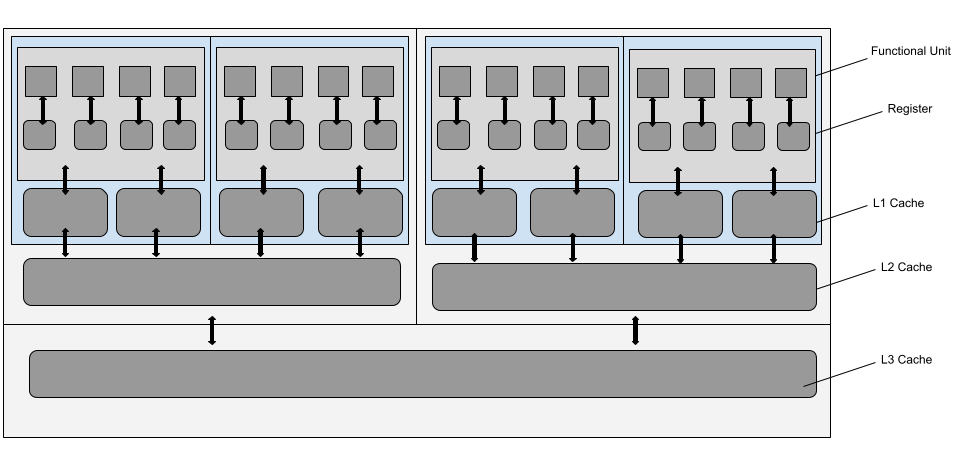
\includegraphics[width=0.75\linewidth]{Processors & Memory Hierarchy Diagram.png}
\end{figure}

    One error programmers may face while designing parallel algorithms is a \textbf{race}. A race happens when two concurrent tasks access the same memory location without proper synchronization and one of the tasks writes to the location. For example, imagine that there exists some variable $X=0$. Task A's job is to perform $X+=1$. Task B's job is to perform $X+=2$. Say now that Task A and Task B read the value of $X$ at the same time (they both get 0). Using that information, Task A adds $0+1$ and writes that value to $X$. Imagine now that Task B finishes after Task A, so it writes $0+2$ to $X$. Even though Task A and Task B were specified sequentially by the programmer so that the end value of $X$ should be 3, both jobs raced, and Task B got the final say. Another type of error is the \textbf{deadlock} in which at least two tasks wait for each other and cannot resume until the other task proceeds. They end up both waiting forever. Another problem that may arise in parallel programming is a \textbf{load imbalance}, when work is distributed unevenly among workers. To avoid such an issue, the overall work should be broken into more smaller tasks than there are workers so that they can be spread out more equally. 

    



\end{document}



